\documentclass{beamer}

\usetheme{Madrid}      % 内置主题(推荐新手使用)
\useoutertheme{miniframes} % 外层主题:横向小方块目录条
% \usetheme{Frankfurt}
% \usepackage[x11names]{xcolor}  % 加载扩展色库
% \usecolortheme[named=OliveDrab3]{structure}  % 柔和绿色
\usepackage{graphicx}
\usepackage{amsmath}
\usepackage{caption}

\title{Wavelet Transform for Image Processing}
\author{
\texorpdfstring{
Zhang Jinrui\thanks{alternative email:zhangjr1022@mails.jlu.edu.cn}
\\
He Jiashun
\\
Meng Jingyuan
\\
Jiang Zishen
\\
Mo Zian
}
{
Zhang Jinrui\thanks{alternative email:zhangjr1022@mails.jlu.edu.cn}
,
He Jiashun
,
Meng Jingyuan
,
Jiang Zishen
,
Mo Zian
}
}
\date{\today}

\begin{document}

\frame{\titlepage}  % 首页封面

\section{Pre-Processing}
% 步骤 1:图像加载与灰度转换
\begin{frame}{1. Image Loading and Grayscale Conversion}
    \begin{block}{Step Explanation}
        The image is loaded using a Python imaging library and converted to grayscale. \\
        This reduces data complexity and focuses analysis on structural content.
    \end{block}

    \vspace{0.5cm}
    \begin{columns}
        \column{0.5\textwidth}
        \centering
        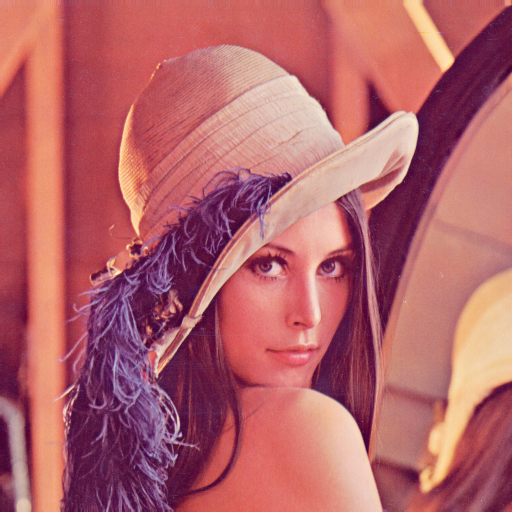
\includegraphics[width=\linewidth]{fig/lena.jpg}
        \captionof{figure}{Original Color Image}

        \column{0.5\textwidth}
        \centering
        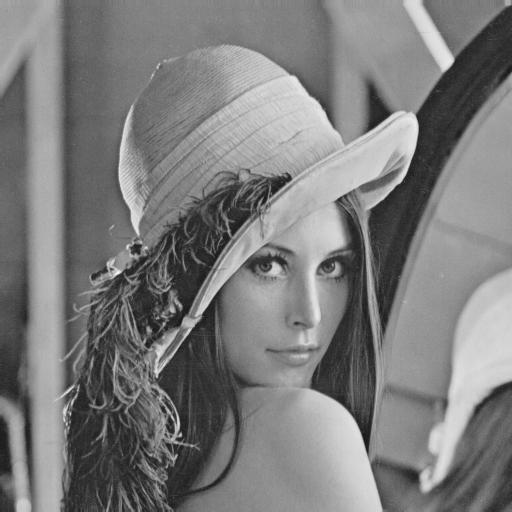
\includegraphics[width=\linewidth]{fig/gray.jpg}
        \captionof{figure}{Grayscale Converted Image}
    \end{columns}
\end{frame}

% 步骤 2 和 3:缩放和居中裁剪
\begin{frame}{2. Rescaling and 3. Centered Cropping}
    \begin{block}{Rescaling with Aspect Ratio Preservation}
        The image is resized using high-fidelity interpolation to ensure one side reaches the target length ($2^N$), without distortion. \\
        The resized image is cropped to $2^N \times 2^N$, ensuring input uniformity without compromising important visual features.
    \end{block}

    \vspace{0.3cm}
    \begin{columns}
        \column{0.5\textwidth}
        \centering
        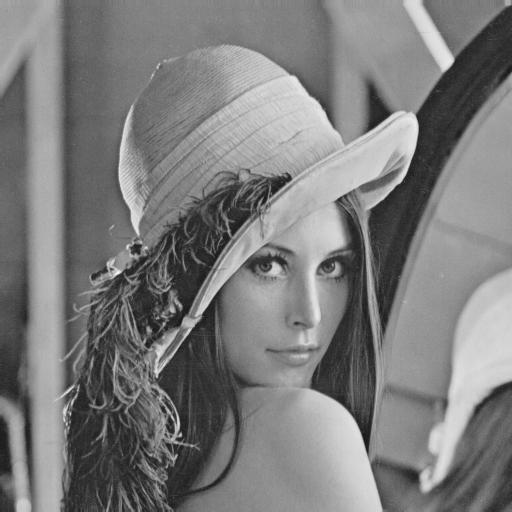
\includegraphics[width=\linewidth]{fig/gray.jpg}
        \captionof{figure}{Before Rescaling}

        \column{0.5\textwidth}
        \centering
        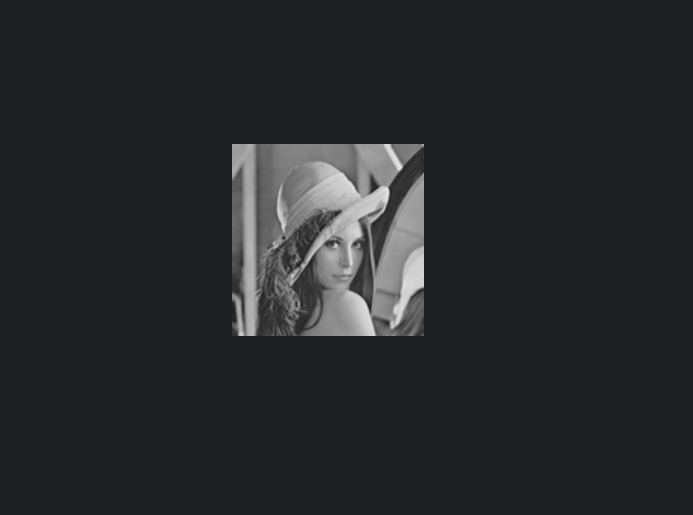
\includegraphics[width=\linewidth, height=5cm]{fig/shuoxiao.png}
        \captionof{figure}{After Rescaling ($2^N$ Side)}
    \end{columns}
\end{frame}

% 步骤 4:矩阵输出
\begin{frame}{4. Matrix Output}
    \begin{block}{Step Explanation}
        The final image is converted into a matrix format suitable for: \\
        $\boldsymbol{\cdot}$ Mathematical operations (e.g., wavelet transforms) \\
        $\boldsymbol{\cdot}$ Storage and machine learning integration
    \end{block}

    \vspace{1cm}
    \centering
    \begin{tabular}{|c|c|c|}
        \hline
        128 & 135 & 142 \\
        \hline
        130 & 138 & 145 \\
        \hline
        125 & 132 & 139 \\
        \hline
    \end{tabular} \\
    \vspace{0.5cm}
    \small{Example of 3x3 image matrix (simplified)}
\end{frame}

% 步骤 5:从矩阵还原图像
\begin{frame}{5. Convert Matrix Information into an Image}
    \begin{block}{Concept}
        Each matrix element represents the gray value of a pixel. Using this matrix, we can reconstruct the grayscale image.
    \end{block}

    \vspace{0.3cm}
    \begin{columns}
        \column{0.5\textwidth}
        \centering
        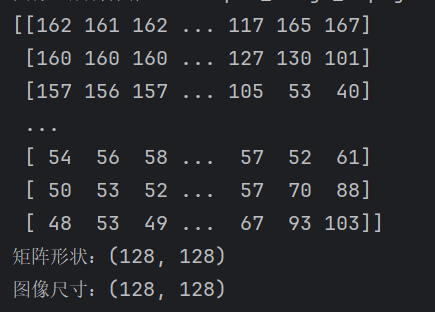
\includegraphics[width=\linewidth]{fig/matrix_information.png}
        \captionof{figure}{Matrix Information}

        \column{0.5\textwidth}
        \centering
        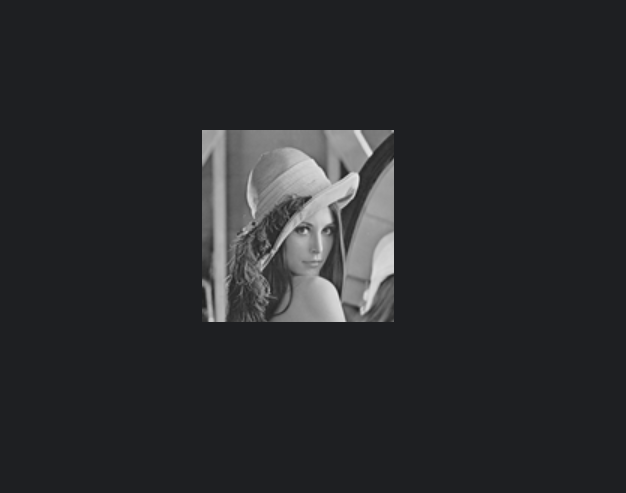
\includegraphics[width=\linewidth]{fig/The_corresponding_image.png}
        \captionof{figure}{Reconstructed Image}
    \end{columns}
\end{frame}

\section{Haar Compression}
\begin{frame}
    \frametitle{Standard Haar Decomposition}
    \begin{itemize}
        \item sdlfkj
        \item sDF
        \item sdf
    \end{itemize}
\end{frame}
\begin{frame}
    \frametitle{sfdfg}
    \begin{itemize}
        \item sdlfkj
        \item sDF
        \item sdf
    \end{itemize}
\end{frame}
\begin{frame}
    \frametitle{sadsgkjh}
    \begin{itemize}
        \item sdlfkj
        \item sDF
        \item sdf
    \end{itemize}
\end{frame}
\begin{frame}
    \frametitle{sdf}
    \begin{itemize}
        \item sdlfkj
        \item sDF
        \item sdf
    \end{itemize}
\end{frame}

\section{Meng Jingyuan}
\begin{frame}
    \frametitle{sadsgkjh}
    \begin{itemize}
        \item sdlfkj
        \item sDF
        \item sdf
    \end{itemize}
\end{frame}

\section{Haar Compression Augmented}
\begin{frame}
    \frametitle{Basic Idea}
    \begin{itemize}
        \item \[
                  \sum_{k=1}^{n}\hat{l}_k^4
                  \geq
                  (\sum_{k=1}^{n}\hat{l}_k^2)^2
                  =
                  (\sum_{k=1}^{n}l_k^2)^2
              \]
        \item \[
                  \min_{\hat{l}_k\in l^2 st. \sum_{k=1}^{n}\hat{l}_k^2=\sum_{k=1}^{n}l_k^2}(-\sum_{k=1}^{n}\hat{l}_k^4)
              \]
    \end{itemize}
\end{frame}
\begin{frame}
    \frametitle{Basic Idea}
    \begin{itemize}
        \item 	\begin{figure}
                  \centering
                  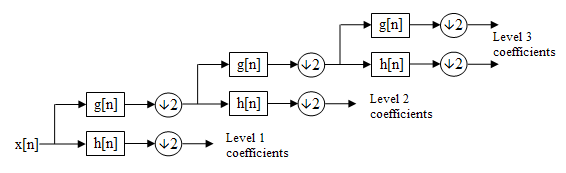
\includegraphics[width=0.8\textwidth]{fig/Wavelets_-_Filter_Bank.png}
                  \caption{Cascading}
                  \label{fig:Cascading}
              \end{figure}
        \item \[
                  \min_{\Phi}(-\sum_{k=1}^{n}\hat{l}_k^4)
              \]
        \item Condense the energy to as less coefficients as possible.
    \end{itemize}
\end{frame}
\begin{frame}
    \frametitle{Results}
    \begin{itemize}
        \item
              \begin{figure}[ht!]
                  \centering
                  \begin{minipage}{0.45\textwidth}
                      \centering
                      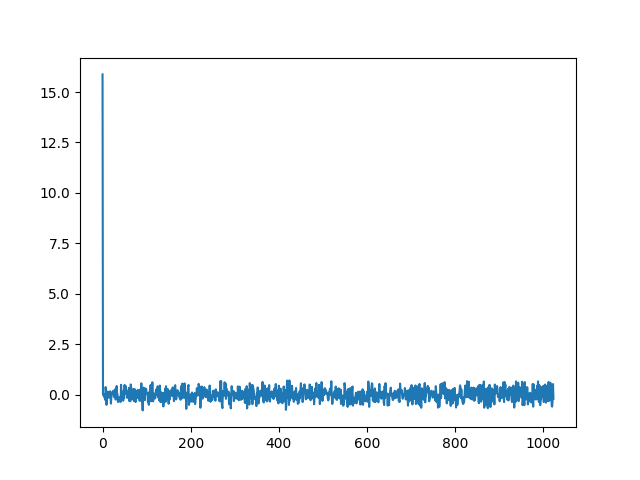
\includegraphics[width=0.9\textwidth]{fig/HaarAugmented1D_freq.png} % first figure itself
                      \caption{Haar 2x2 filter bank random input. Compression Rate 0.2568}
                      \label{fig:Haar}
                  \end{minipage}\hfill
                  \begin{minipage}{0.45\textwidth}
                      \centering
                      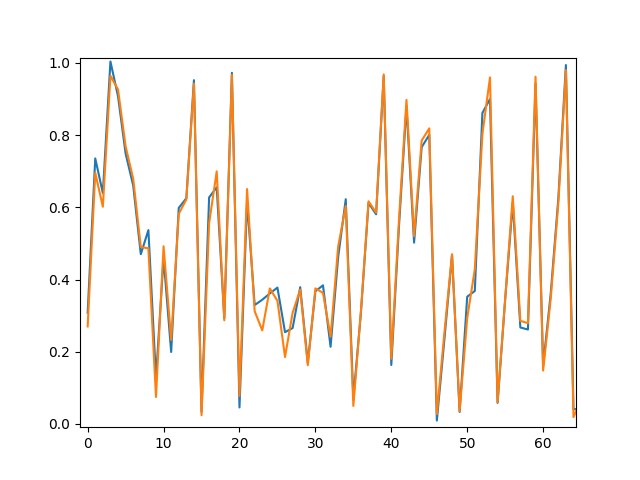
\includegraphics[width=0.9\textwidth]{fig/HaarAugmented1D_rec.png} % second figure itself
                      \caption{Haar 2x2 filter bank random input.Total average energy loss 0.0009}
                  \end{minipage}
              \end{figure}
              %   \begin{figure}
              %       \centering
              %       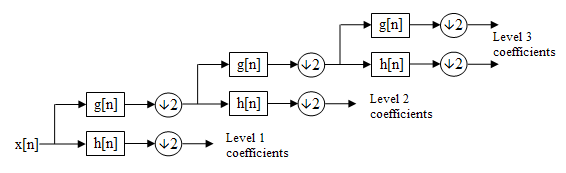
\includegraphics[width=0.8\textwidth]{fig/Wavelets_-_Filter_Bank.png}
              %       \caption{Siakam won 2025 NBA eastern conference finals MVP}
              %       \label{fig:Siakam}
              %   \end{figure}
              % \item Random sequence would have large information entropy so it have a low compression rate.
    \end{itemize}
\end{frame}
\begin{frame}
    \frametitle{Results}
    \begin{itemize}
        \item
              \begin{figure}[ht!]
                  \centering
                  \begin{minipage}{0.45\textwidth}
                      \centering
                      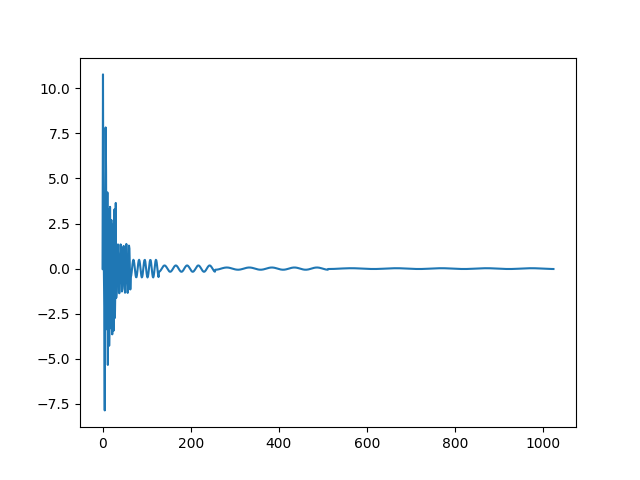
\includegraphics[width=0.9\textwidth]{fig/HaarAugmented1D_sin_freq.png} % first figure itself
                      \caption{Haar 2x2 filter bank sin input frequency. Compression Rate 0.9287}
                      \label{fig:Haar_sin}
                  \end{minipage}\hfill
                  \begin{minipage}{0.45\textwidth}
                      \centering
                      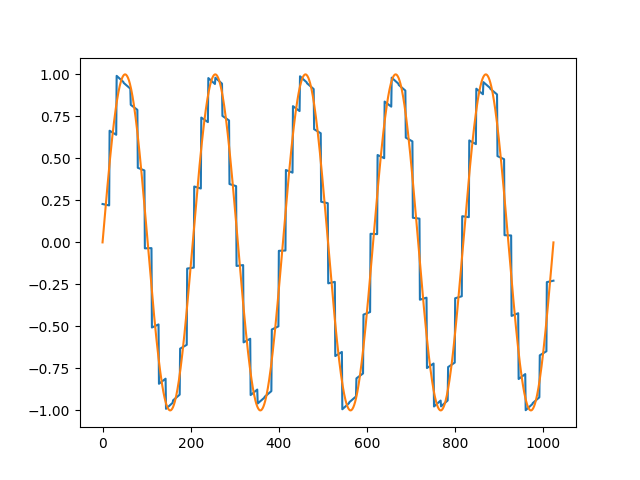
\includegraphics[width=0.9\textwidth]{fig/HaarAugmented1D_sin_rec.png} % second figure itself
                      \caption{Haar 2x2 filter bank sin input reconstruction.Total average energy loss 0.0104}
                  \end{minipage}
              \end{figure}
              %   \begin{figure}
              %       \centering
              %       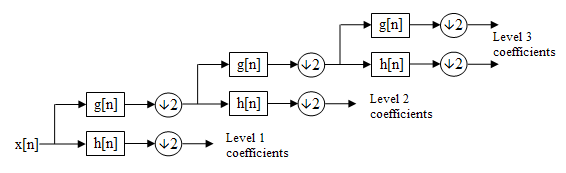
\includegraphics[width=0.8\textwidth]{fig/Wavelets_-_Filter_Bank.png}
              %       \caption{Siakam won 2025 NBA eastern conference finals MVP}
              %       \label{fig:Siakam}
              %   \end{figure}
              % \item A smooth signal have small information entropy, so will have a high compression rate.
    \end{itemize}
\end{frame}
\begin{frame}
    \frametitle{Results}
    \begin{itemize}
        \item
              \begin{figure}[ht!]
                  \centering
                  \begin{minipage}{0.45\textwidth}
                      \centering
                      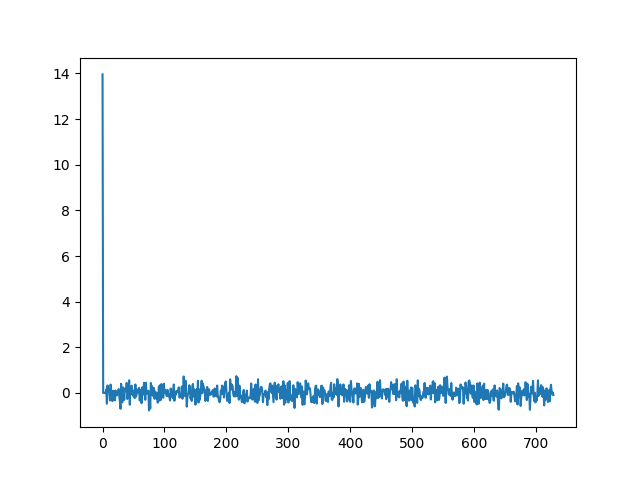
\includegraphics[width=0.9\textwidth]{fig/Haar3Augmented1D_freq.png} % first figure itself
                      \caption{Haar 3x3 filter bank random input. Compression Rate 0.1906}
                      \label{fig:Haar3}
                  \end{minipage}\hfill
                  \begin{minipage}{0.45\textwidth}
                      \centering
                      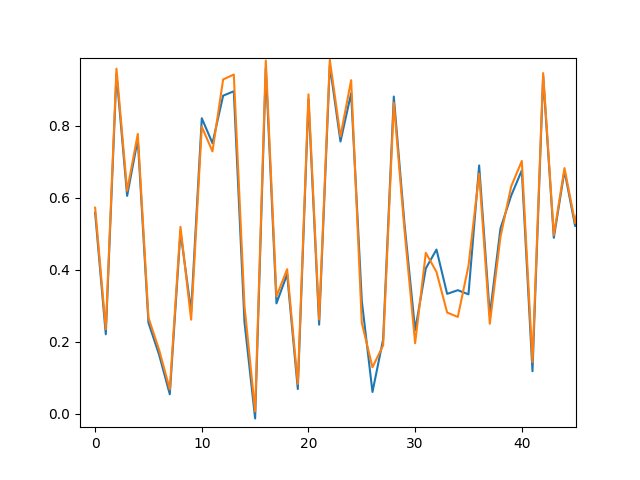
\includegraphics[width=0.9\textwidth]{fig/Haar3Augmented1D_rec.png} % second figure itself
                      \caption{Haar 3x3 filter bank random input.Total average energy loss 0.0008}
                  \end{minipage}
              \end{figure}
              %   \begin{figure}
              %       \centering
              %       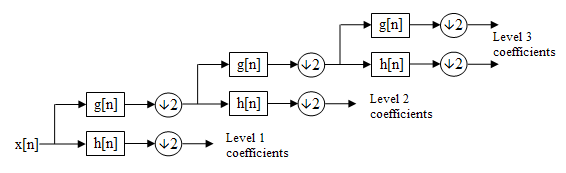
\includegraphics[width=0.8\textwidth]{fig/Wavelets_-_Filter_Bank.png}
              %       \caption{Siakam won 2025 NBA eastern conference finals MVP}
              %       \label{fig:Siakam}
              %   \end{figure}
              % \item same random sequence same reason.
    \end{itemize}
\end{frame}
\begin{frame}
    \frametitle{Results}
    \begin{itemize}
        \item
              \begin{figure}[ht!]
                  \centering
                  \begin{minipage}{0.45\textwidth}
                      \centering
                      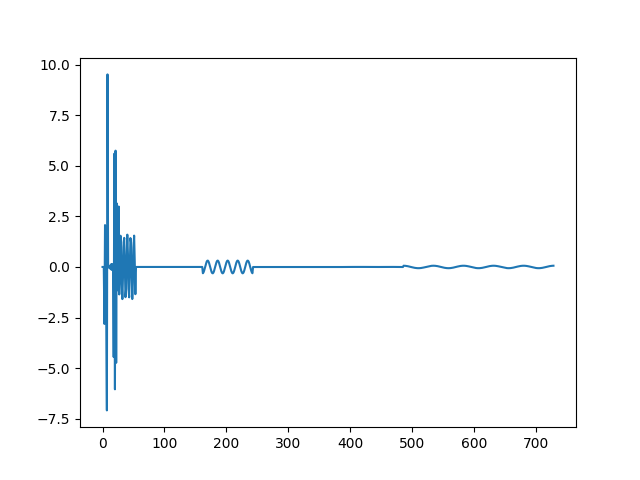
\includegraphics[width=0.9\textwidth]{fig/Haar3Augmented1D_sin_freq.png} % first figure itself
                      \caption{Haar 3x3 filter bank sin input frequency. Compression Rate 0.7750}
                      \label{fig:Haar3_sin}
                  \end{minipage}\hfill
                  \begin{minipage}{0.45\textwidth}
                      \centering
                      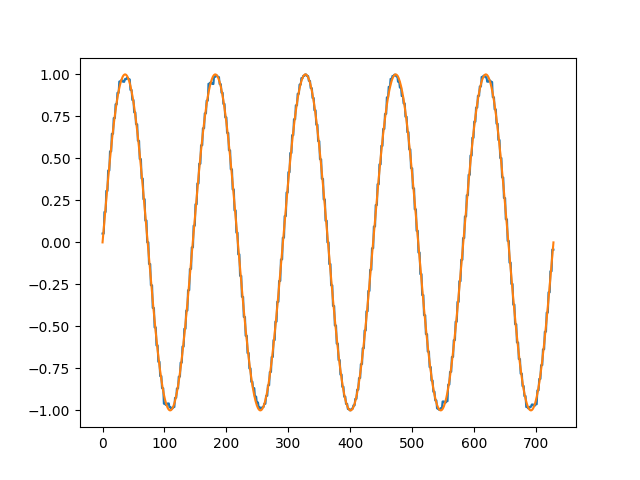
\includegraphics[width=0.9\textwidth]{fig/Haar3Augmented1D_sin_rec.png} % second figure itself
                      \caption{Haar 3x3 filter bank sin input reconstruction.Total average energy loss 0.0007}
                  \end{minipage}
              \end{figure}
              %   \begin{figure}
              %       \centering
              %       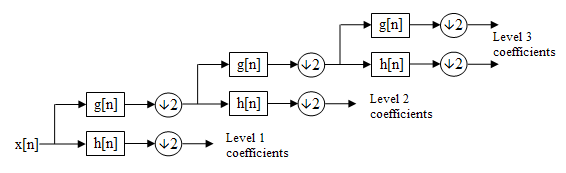
\includegraphics[width=0.8\textwidth]{fig/Wavelets_-_Filter_Bank.png}
              %       \caption{Siakam won 2025 NBA eastern conference finals MVP}
              %       \label{fig:Siakam}
              %   \end{figure}
              % \item same smooth signal same reason.
    \end{itemize}
\end{frame}

\section{Equivalent Characterizations}

\begin{frame}{Main Theorem -- Four Equivalent Statements}
    The following are equivalent:

    \begin{enumerate}
        \item The filter bank $(\{\tilde u_\ell\},\{u_\ell\})$ has PR.
        \item $\displaystyle\frac12\sum_{\ell=0}^{s} S_{u_\ell}T_{\tilde u_\ell}v = v$ for all $v\in\ell(\mathbb{Z})$.
        \item The identity holds for $v=\delta$ and $v=\delta(\cdot-1)$.
        \item Frequency-domain identities for all $\omega\in\mathbb{R}$:
              \[
                  \sum_{\ell=0}^{s}\overline{\hat{\tilde u}_\ell(\omega)}\hat u_\ell(\omega)=1,
              \]
              \[
                  \sum_{\ell=0}^{s}\overline{\hat{\tilde u}_\ell(\omega)}\hat u_\ell(\omega+\pi)=0.
              \]
    \end{enumerate}
\end{frame}


\subsection*{Proof Sketch-Implications}

\begin{frame}{(i) $\Rightarrow$ (ii) $\Rightarrow$ (iii)}
    Trivial inclusions:
    \[
        \ell_0(\mathbb{Z})\subseteq \ell(\mathbb{Z})\quad\text{and}\quad \delta,\delta(\cdot-1)\in\ell_0(\mathbb{Z}).
    \]
\end{frame}

\begin{frame}{(iii) $\Rightarrow$ (iv)}
    \begin{enumerate}
        \item \textbf{Frequency Domain Conversion:} Using Fourier transforms of $T_{\tilde{u}_\ell}$ and $S_{u_\ell}$:
              \[
                  \widehat{T_{\tilde{u}_\ell} v}(\omega) = \hat{v}(\omega/2)\overline{\hat{\tilde{u}}_\ell(\omega/2)} + \hat{v}(\omega/2+\pi)\overline{\hat{\tilde{u}}_\ell(\omega/2+\pi)},
              \]
              \[
                  \widehat{S_{u_\ell} w}(\omega) = \hat{w}(2\omega)\hat{u}_\ell(\omega).
              \]

        \item \textbf{Substitute Basis Signals:} Plugging $v = \delta$ ($\hat{v}=1$) and $v = \delta(\cdot-1)$ ($\hat{v}=e^{-i\omega}$) into the PR condition yields the system:
              \[
                  \sum_{\ell=0}^s \overline{\hat{\tilde{u}}_\ell(\omega)}\hat{u}_\ell(\omega) + \sum_{\ell=0}^s \overline{\hat{\tilde{u}}_\ell(\omega+\pi)}\hat{u}_\ell(\omega+\pi) = 2,
              \]
              \[
                  \sum_{\ell=0}^s \overline{\hat{\tilde{u}}_\ell(\omega)}\hat{u}_\ell(\omega) - \sum_{\ell=0}^s \overline{\hat{\tilde{u}}_\ell(\omega+\pi)}\hat{u}_\ell(\omega+\pi) = 0.
              \]

        \item \textbf{Solve System:} Adding and subtracting these equations gives condition (iv).
    \end{enumerate}
\end{frame}

\begin{frame}{(iv) $\Rightarrow$ (ii) and (ii) $\Rightarrow$ (i)}
    \begin{itemize}
        \item (iv) $\Rightarrow$ (ii): Condition (iv) implies the frequency identity holds for all $v \in \ell_0(\mathbb{Z})$ by linearity of Fourier transform.
        \item (ii) $\Rightarrow$ (i):  {Localization Argument:} For any $v \in \ell(\mathbb{Z})$, truncate to local signal $v_n \in \ell_0(\mathbb{Z})$ using finite support of filters. Apply (ii) to show:
              \[
                  v(n) = \frac{1}{2}\sum_{\ell=0}^s [S_{u_\ell} T_{\tilde{u}_\ell} v](n).
              \]
    \end{itemize}
\end{frame}

\end{document}
